I% Chapter Template

\chapter{Vector Structure and Operations} % Main chapter title

\label{VectorStructure} % Change X to a consecutive number; for referencing this chapter elsewhere, use \ref{ChapterX}

\lhead{Vector Structure. \emph{Vector Structure}} % Change X to a consecutive number; this is for the header on each page - perhaps a shortened title

%----------------------------------------------------------------------------------------
%	SECTION - Radix Balanced Vectors
%----------------------------------------------------------------------------------------

\section{Radix Balanced Vectors}

% vector as a wrappers for the tree
The current immutable vector implementation\cite{scalaVector211} of the Scala Collections is wrapper around an RB-Tree. The vector implements the methods of \texttt{IndexedSeq} based on a set of core efficient operations on RB-Trees.

%-----------------------------------
%	SUBSECTION - Tree structure
%-----------------------------------

\subsection{Tree structure}
% describe tree: balancing, filling, block sizes
% hint why radix?
% why structure helps with operations implementation 
The RB-Tree structure is shallow densely filled tree where elements are located only in the leafs and on the left side. Each node of the three has the same amount of children and the leaf have as many elements. Currently this number is 32, but could be any power of 2 to be able to have efficient radix based implementations (see \ref{ComputingIndices}). Figure \ref{badix_balanced} shows this structure for $m$ children on each node. 

\begin{figure}[h!]
  \centering
  \includegraphics[width=\textwidth]{Figures/Radix_Balanced}
  \caption{Radix Balanced Tree Structure}
   \label{badix_balanced}
\end{figure}

All nodes are represented with immutable\footnote{Immutable arrays are just mutable arrays that do not get updated after initialisation.} \texttt{Array[AnyRef]}, as this is the most compact representation for the structure and will help performance by the use of JVM primitive operations (see \ref{InPractice}). Because branches and leafs are represented the same way, the vector also need to know the hight of the RB-Tree. It is kept in the \texttt{depth} field. This height will alway be upper bounded by $log_{32}(size-1)+1$ for nodes of 32 branches. Therefore the tree is quite shallow and the complexity to traverse it is considered as effectively constant when taking into account that the size will never exude the maximum index representable with \texttt{Int}.

To have trees that will contain an amount of elements that does not match a full tree we fill first the elements from the left. The branches on the right that do not contain any element in any of it's leafs are not allocated (left as empty references or truncated arrays). For example the tree that would hold 1056 elements in figure \ref{badix_balanced_32} would have empty subtrees on the right of the nodes on the rightmost branch. To never access elements that are outside of a the trees right bound, the vector has an \texttt{endIndex} field that point to that last index. With this it is possible to have efficient implementations of  \texttt{take} and \texttt{append} (see \ref{Operations}).

\begin{figure}[h!]
  \centering
  \includegraphics[width=0.4\textwidth]{Figures/Radix_Balanced_32}
  \caption{Radix Balanced Tree Structure with nodes of size 32 filled with 1056 elements.}
   \label{badix_balanced_32}
\end{figure}

Additionally, to have efficient implementation of \texttt{drop} and \texttt{prepend} operations (see \ref{Operations}), the vector defines a \texttt{startIndex} field that points to the first element in the tree that is actually used in the vector. The tree is left empty on the left of the first element. Arrays on the nodes of the left branch must be allocated wit the full size. As such, the tree structure is logically still full on the left but element are never access due to a shift if the index using the \texttt{startIndex}. Therefore radix indexing is still possible.

%-----------------------------------
%	SUBSECTION - Operations
%-----------------------------------
\subsection{Operations}
\label{Operations}
% List core operations
The immutable \texttt{Vector} \cite{scalaVector211} is a subtype of \texttt{IndexedSeq} in the current Scala collections, as such it implements all operations defined on it. Most operations are implemented using a set of core operations that can be implemented efficiently on RB-Trees, those operations are: \texttt{apply}, \texttt{updated}, \texttt{append}, \texttt{prepend}, \texttt{drop} and \texttt{take}. 

% performance log_{32}(n) -> effective constant time
The performances of most operations on RB-Trees have a computational complexity of $O(log_{32}(n))$, equivalent to the height of the tree. This is usually referred as effective constant time because for 32 bit signed indices the height of the tree will bounded by a small constant (6.2 in the case of books of size 32). This bound is reasonable to ensure that in practice the operations behave like constant time operations.  
 
% naive implementation just as high level guide
% hint of displays and transient states
In this section the operations will be presented on a high level\footnote{Ignoring some pieces of code like casts, return types, type covariance, among others.} and without optimisation. These reflect the worst case scenario or the base implementation that is used before adding optimizations (see chapter \ref{Optimizations}). To improve performance of some operations, displays are used on branches of the RB-Tree (see section \ref{sec:Displays}). To improve the complexity of operations to amortized constant time (instead of effective constant time\footnote{In this context, effective constant time has a large but bounded constant time complexity, while amortized constant time tends to have a bound closer to a one level tree update.}) for some operation sequences the vectors are augmented with transient states.

%-----------------------------------
%	SUBSUBSECTION - Apply
%-----------------------------------

\subsubsection{Apply}
\label{sec:apply}
% used in head and last
The \texttt{apply} operation in indexed sequences is defined as the operation that gets the element located at some index. This is the main element access method and it is used in other methods such as \texttt{head} and \texttt{last}.

\begin{lstlisting}[frame=single]
def apply(index: Int): A = {
  def getElem(node: Array[AnyRef], depth: Int): A = {
    val indexInNode = // compute index
    if(depth == 1) node(indexInNode)
    else getElem(node(indexInNode), depth-1) 
  }
  getElem(vectorRoot, vectorDepth)
}
\end{lstlisting}

% performance log_{32}(n), hint of displays
The base implementation on RB-Trees of this operation requires a simple traversal from the root to the leaf containing the element. Where the path taken is defined by the index of the element and extracted using some efficient bitwise operations (see section \ref{ComputingIndices}). With this traversal of the tree, the complexity of the \texttt{apply} operation is $O(log_{32}(n))$. This complexity can be reduced for some subset of elements by adding displays.


%-----------------------------------
%	SUBSUBSECTION - Updated
%-----------------------------------

\subsubsection{Updated}
\label{sec:updated}
% base implementation needs to update the whole branch
The \texttt{updated} method returns a new immutable \texttt{Vector} with one updated element at a given index. This is the core operation to modify the contents of the vector. 

On immutable RB-Trees the updated operation has to recreate the whole branch from the root to the element being updated. The update of the leaf creates a fresh copy of the leaf with the updated element. Then the parent of the leaf also need to create a new node with the updated reference to the new leaf, and so on up to the root. 

\begin{lstlisting}[frame=single]
def updated(index: Int, elem: A) = {
  def updatedNode(node: Array[AnyRef], depth: Int) = {
    val indexInNode = // compute index
    val newNode = copy(node)
    if(depth == 1) {
      newNode(indexInNode) = elem
    } else {
      newNode(indexInNode) = 
        updatedNode(node(indexInNode), depth-1)
    }
    newNode
  }
  new Vector(updatedNode(vectorRoot, vectorDepth), ...)
}
\end{lstlisting}

% with transient states, local updates can be amortised
Therefore the complexity of this operation is $O(log_{32}(n))$, for the traversal and creation of each node in the brach. This operation can be improved to have amortized constant time updates for local updates using displays with transient states. This way the parent nodes are only updated lazily when absolutely necessary. For example, if some leaf has all it's elements updated from left to right, the leaf will be copied as many times as there are updates, but the parent of that leaf does not change during those operations.

%-----------------------------------
%	SUBSUBSECTION - Additions
%-----------------------------------

\subsubsection{Extentions}
The main operations to extend an immutable \texttt{Vector} are \texttt{append} and \texttt{prepend} a single element. Those operations are considered the main ones because they have efficient implementations on RB-Trees. Other operations like \texttt{concatenated} are also present, but usually avoided because of performance.


\paragraph{Append}
% base implementation needs to update the whole branch
To append an element on the tree there are two main cases, the last leaf of the tree is not full or it is full. If the last leaf is not full the element is inserted at the end of it and all nodes of the last branch are updated. Or, if the leaf is full we must find the lowest node in the last branch where there is sill room left for a new branch. Then a new branch is appended to it, down to the a new leaf with the element being appended. 

In both cases the new \texttt{Vector} object will have the end index increased by one. When the root is full, the depth of the vector will also increase by one.

\begin{lstlisting}[frame=single]
def :+(elem: A): Vector[A] = {
  def append(node: Array[AnyRef], depth: Int) = {
    if (depth == 1) 
      copyLeafAndAppend(node, elem)
    else if (!isTreeFull(node.last, depth-1)) 
      copyAndUpdateLast(node, append(node.last, depth-1))
    else
      copyBranchAndAppend(node, newBranch(depth-1))
  }
  def createNewBranch(depth: Int): Array[AnyRef] = {
    if (depth == 1) Array(elem)
    else Array(newBranch(depth-1))
  }
  if(!isTreeFull(root, depth))) 
    new Vector(append(root, depth), depth, ...)
  else 
    new Vector(Array(root, newBranch(depth)), depth+1, ...)
}
\end{lstlisting}

Where the \texttt{isTreeFull} operation computes the answer using efficient bitwise operations on the end index of the vector.

% performance log_32(n), hint of transient to amortise consecutive appends are amortised
Due to the update of all nodes in the last branch, the complexity of this operation is $O(log_{32}(n))$. This complexity can be amortized to constant time using displays with transient states for consecutive append operations on the vector (see section \ref{sec:DisplaysTransient}).

\paragraph{Prepend}
% base implementation needs to update the whole branch
The key to be able to prepend  elements to the tree is the additional \texttt{startIndex} that the vector keeps. Without this it would be impossible to prepend an element to the vector without a full copy of the vector to rebalance the RB-Tree. The operation can be split into to cases depending on the value of the start index.

% shift top and start index
The first case is to prepend an element on a vector that start at index 0. If the root is full, create a new root on top with the old root as branch at index 1. If there is still space in the root, shift branches in the root by one to the right. In both sub\-cases, create a new branch containing nodes of size 32, but with only the last branch assigned. Put the element in the last position of this newly created branch and set the start index of the vector to that index in the tree.

The second case is to prepend an element on a vector that has a non zero start index. Follow the branch of the start index minus one from the root of the tree. If it reaches the a leaf, prepend the element to that leaf. If it encounters an inexistent branch, create it by putting the element in its rightmost position and leaving the rest empty. In both sub\-cases update the parent nodes up to the root.

The new \texttt{Vector} object will have an updated start index and end index. to account for the changes in the structure of the tree. It may also have to increase the depth of the vector if the start index was previously zero. 

\begin{lstlisting}[frame=single]
def +:(elem: A): Vector[A] = {
  def prepended(node: Array[AnyRef], depth: Int) = {
    val indexInNode = // compute index
    if (depth == 1) 
      copyAndUpdate(node, indexInNode, elem)
    else 
      copyAndUpdate(node, indexInNode, 
                prepended(node(indexInNode), depth-1))
  }
  def newBranch(depth: Int): Array[AnyRef] = {
    val newNode = new Array[AnyRef](32)
    newNode(31) = 
      if (depth == 1) elem 
      else newBranch(depth-1)
    newNode
  }
  if (startIndex==0) {
    new Vector(Array(newBranch(depth), root), depth+1, ...)
  } else {
    new Vector(prepended(root, depth), depth, ...)  
  }
}
\end{lstlisting}

% performance log_32(n), hint of transient to amortise consecutive prepends are amortised
Due to the update of all nodes in the first branch, the complexity of this operation is $O(log_{32}(n))$. This complexity can be amortized to constant time using displays with transient states for consecutive prepend operations on the vector (see section \ref{sec:DisplaysTransient}).


\paragraph{Concatenation}
% describe high level implementation in vector
Given that elements in an RB-Tree are densely packed, implementations for concatenation and insert will need to rebalance elements to make them again densely packed. In the case of concatenation there are three options to join the two vectors: append all elements of the RHS vector to the LHS vector, prepend all elements from the LHS vector to the RHS vector or simply reconstruct a new vector using a builder. The append and prepend options are used when on of the vectors is small enough in relation to the other one. When vectors become large, the best option is the one with the builder because it avoids creating one instance of the vector each time an element is added.

% performance O(n)
The computational complexity of the concatenation operation on RB-Trees for vectors lengths $n1$ and $n2$ is $O(n1 + n2)$ in general. In the special case where $n1$ or $n2$ is small enough the complexity becomes $O(min(n1,n2)*log_{32}(n1+n2))$, the complexity of repeatedly appending or prepending an element. This last one can be amortised to $min(n1,n2)$ using displays and transient states. 

%-----------------------------------
%	SUBSUBSECTION - Splits
%-----------------------------------

\subsubsection{Splits}
% used in tail, init, take, takeRight, drop, dropRight
The core operations to remove elements in a vector are the \texttt{take} and \texttt{drop} methods. They are used to implement may other operations like \texttt{splitAt}, \texttt{tail}, \texttt{init}, ...

% describe implementation in vector
Take and drop have a similar implementation. The first step is traversing the tree the leaf where the cut will be done. Then the branch is copied and cleared on one side. The whole branch is not necessarily copied, if the resulting tree is shallower the nodes on the top that would have only one child are removed. Finally, the \texttt{startIndex} and \texttt{endIndex} are adjusted according to the changes on the tree.

% performance log_32(n) 
The computational complexity of any split operation is $O(log_{32}(n))$ due to the traversal and copy of nodes on the branch where the cut index is located.


%----------------------------------------------------------------------------------------
%	SECTION - Parallel Vectors
%----------------------------------------------------------------------------------------

\section{Parallel Vectors}
% how are they paralellized (wraps an vector)
% fork-join pool
Parallel vector or \texttt{ParVector} are just a wrapper around the normal \texttt{Vector} object that uses the parallel collections API instead of the normal collections API. With this, operations on collections get executed transparently on fork-join thread pools rather that on the main thread. The only additional implementation requirements are a \texttt{Splitter} and \texttt{Combiner} that are used to manage the execution distribution of work. 

% why do they suffer performance wise (no efficient concat)
\texttt{ParVector} has performance drawbacks on the \texttt{Combiner} because this one requires an efficient concatenation implementation. To avoid excessive overhead on concatenation the current implementation does it lazily, which comes with a second drawback on loss of parallelism of the combine operation.

%-----------------------------------
%	SUBSUBSECTION - Splitter
%-----------------------------------

\subsection{Splitter (Iterator)}
% split into half 
To divide the work into tasks for thread pool, a splitter is used to iterate over all elements of the collection. Splitters are a special kind of iterator that can be split at any time into some partition of the remaining elements. In the case of sequences the splitter should retain the original order. The most common implementation consists in dividing the remaining elements into two half. 

The current implementation of the immutable parallel  vector \cite{scalaParVector211}  uses the common division into 2 parts for it splitter. The drop and take operations are used divide the vector for the two new splitters.

%-----------------------------------
%	SUBSUBSECTION - Combiner
%-----------------------------------

\subsection{Combiner (Builder)}
% lazy combiner
Combiners are used to merge the results from different tasks (in methods like map, filter, collect, ...) into the new collection. Combiners are a special kind of builder that is able to merge to partial results efficiently. When it's impossible to implement efficient combination operation, usually a lazy combiner is used. The lazy combiner is one keeps all the it's sub-combiners in an array buffer and only when the end result is needed they are combined. This is a fairly efficient implementation but does not take full advantage of parallelism. 

The current implementation of the immutable parallel vector \cite{scalaParVector211} use the lazy approach because of it's inefficient concatenation operation. One of the consequences of this is that the parallel operations will always be bounded by this sequential combination of elements, which can be beaten by the sequential version in many cases.
 

%----------------------------------------------------------------------------------------
%	SECTION - Relaxed Radix Balanced Vectors
%----------------------------------------------------------------------------------------

\section{Relaxed Radix Balanced Vectors}

The implementation for RRB vectors proposed consists in replacing the wrapped RB-Tree by an RRB-Tree and augmenting the operations accordingly while trying to maintain the performance of RB-Tree operations. The structure of the RRB-Trees doesn't ensure by itself that the tree height is bounded, this is something that the implementation of the operations must ensure. 

%-----------------------------------
%	SUBSECTION - Tree structure
%-----------------------------------

\subsection{Relaxed Tree structure}
% describe tree: balancing, filling, block sizes
An RRB-Tree is an generalisation of an RB-Tree where there is an additional kind of node. This is the unbalanced node, it is a node that does not require the it's children to be full. Leaf nodes are never considered as unbalanced. For efficiency it will additional have information on the sizes of it's children.

% describe sizes array and where it is kept (change from left to right for indexing simplification)
In an unbalanced node, the sizes are kept in an \texttt{Array[Int]} and attached at the end of the array that contains the children. The sizes array has the same length as the number of children of the node as is shown in figure \ref{Relaxed_Radix_balanced}. This kind of nodes get truncated rather that keep empty branches as all the information that was usually needed on radix operations is now in the sizes.

\begin{figure}[h!]
  \centering
  \includegraphics[width=\textwidth]{Figures/Relaxed_Radix_balanced}
  \caption{Radix Balanced Tree structure}
  \label{Relaxed_Radix_balanced}
\end{figure}

In the RRB-Tree paper \cite{RRBTrees} the sizes are located in the front. They where moved to favour the performance on radix indexing on balanced node rather than on unbalanced nodes sizes. This is based on the assumption that most operation will be executed on balanced nodes.

% mention size of nodes and null sizes
To have an homogenous representation for unbalanced nodes and balanced node, the balanced nodes arrays are extended with one extra empty position at the end. Therefore all the nodes have the same structure and the node is balanced if and only if the last position is empty\footnote{Empty position is just a \texttt{null} reference.}. The leafs do not need this additional data. Figure \ref{Relaxed_radix_example} shows an example of a RRB-Tree that has a combination of balanced an unbalances nodes.

\begin{figure}[h!]
  \centering
  \includegraphics[width=\textwidth]{Figures/Relaxed_radix_example}
  \caption{Concrete example of an RRB-Tree that contains 1090 elements.}
  \label{Relaxed_radix_example}
\end{figure}

As it it possible to represent trees that are not field on the left, the \texttt{startIndex} is removed from the \texttt{Vector} object and assumed to be alway zero. The \texttt{endIndex} is also not strictly necessary but is kept for performance of index bound checks.

%-----------------------------------
%	SUBSECTION - Operations
%-----------------------------------
\subsection{Relaxing the Operations}
% describe how the implementation uses relaxed radix when necessary and uses radix based operation when possible
Form most operations the implementation is relaxed using the same technique. It consist in using a generalised version of the code for RB-Trees that take into account the unbalanced nodes that do not support radix operations. Mainly this consists in changing the way the \texttt{indicesInNode} are computed on unbalanced nodes and their \texttt{clone} operations.
 
To take advantage of radix based code when possible the operations will still call the radix version if the node is balanced. This implies that from a balanced node down the radix based code is executed. Only the unbalanced nodes will have loss in performance due to generalisation and therefore the code executed for a balanced RRB-Tree will tend to be the same as the one for RB-Trees.

% ensuring height bounds
As the RRB-Tree structure does not ensure the bound on the height unless the tree is completely balanced, the operation must ensure that tree respects the $log_{32}(n)$ height. Fortunately there are only three operations that can unbalance a tree: the \texttt{concatenated}, \texttt{prepend} and \texttt{drop} operations. The operations that also modify the structure of the tree like \texttt{append} and \texttt{take} do not add unbalanced nodes but can affect the existing ones.

%-----------------------------------
%	SUBSUBSECTION - Apply
%-----------------------------------
\subsection{Core operations with minor changes}

\paragraph{Apply}
% describe the way to get the node indices in an unbalanced node
The apply operation does not fundamentally change. The only difference is in the way the index of the next branch of a node is computed. If the node is unbalanced the sizes of the tree must be accessed (see section \ref{ComputingIndices}).


%-----------------------------------
%	SUBSUBSECTION - Updated
%-----------------------------------

\paragraph{Updated}
% doesn't change much, the sizes do not need to be updated, they jus need to be copied. Going to the correct position still may needs to access the sizes.
For the \texttt{updated} the changes are simple because the structure of the RRB-Tree will not be affected. The computation of the \texttt{indexInNode} will change to take into account the possibility of unbalanced nodes while traversing down the tree. The \texttt{copy} operation will need to copy the sizes of the node if the node is unbalances. Because the sizes are represented in an immutable array, this copy of sizes is in fact a reference to the same object.

%-----------------------------------

\paragraph{Append}
% difference is that the the sizes may need to be updated
% performance log_32(n), remind hint of transient to amortise consecutive appends are amortised
To append an element on an RRB-Tree it is only necessary to change the \texttt{copyBranchAndAppend},  \texttt{copyAndUpdateLast} and \texttt{createNewBranch} helper functions. The \texttt{copyBranchAndAppend} will additionaly copy the sizes ad append to it a new size with value equal the the old last size plus one. The \texttt{copyAndUpdateLast} will also copy the sizes of the branch and increase the last size by one. The \texttt{createNewBranch} will have to allocate one empty position at the end of the new non leaf nodes of the branch. Note that any new branch created by append will be created as a balanced subtree.

%-----------------------------------

\paragraph{Take}
% describe difference between the implementation (null and shift vs. cut and update size)
This operation needs to take into account the RRB tree traversal scheme to go down to the index. The tree is cut in the same way the RB-Tree is cut with an additional step. When cutting an unbalanced node the sizes of that node are cut at the same index and the last size is adjusted to match the elements in the cut. 

%-----------------------------------

\subsection{Concatenation}
% describe high level implementation in rrbvector
% performance log_32(n)
The concatenation algorithm use on RRB-Vectors is the one proposed in the RRB-Trees paper \cite{RRBTrees}. From a high level, the algorithm merges the rightmost branch of the vector on the LHS with the leftmost branch of the vector on the RHS. While merging the node, there is a rebalancing that is effectuated on each of them to ensure the logarithmic bound on the height of the vector. The RRB version of concatenation has a time complexity of $O(log_{32}(n))$, which is a clear improvement from the RB concatenation that was $O(n)$.
 
%\lstinputlisting[]
\begin{lstlisting}[frame=single]
def concatenate(left: Vector[A], right: Vector[A]) = {
   val newTree = mergedTrees(left.root, right.root)
   val maxDepth = max(left.depth, right.depth)
   if (newTree.hasSingleBranch)
     new Vector(newTree.head, maxDepth)
   else 
     new Vector(newTree, maxDepth+1)
}
def mergedTrees(left: Node, right: Node, depth: Int) {
  if (depth==1) {
    mergedLeafs(left, right)
  } else { 
    val merged = 
      if (depth==2) mergedLeafs(left.last, right.first) 
      else mergedTrees(left.last, right.first, depth-1)
    mergeRebalance(left.init, merged, right.tail)
  }
}
def mergedLeafs(left: Node, right: Node} = {
  // create a balanced new tree of height 2 
  // with all elements in the nodes
}
\end{lstlisting}

%% describe high level algorithm
The concatenation operation starts at the bottom of the branches by merging the leafs into a balanced tree of height 2 using \texttt{mergedLeafs}. Then, for each level on top of it, the newly created merged subtree and the remaining branches on that level will be merged and rebalanced into a new subtree. This new subtree always adds a new level to the tree, even though it might be drop later on. New sizes of nodes are computed each time a node is created based on sizes of children nodes.

%% describe branch rebalancing 
The rebalancing algorithm has two proposed variants. The first consists in completely rebalancing the nodes on the two top levels of the subtree. The second also rebalances the top two level of the subtree but it only rebalance the minimum amount of nodes that ensures the logarithmic bound. The first one leaves the tree better balanced, while the second is faster. More detail on the bounds and complexities can be bound on the RRB-Tree paper \cite{RRBTrees}. The following snippet of code shows a high level implementation of the first variant.

\begin{lstlisting}[frame=single]
def mergeRebalance(left: Node, center: Node, right: Node) {
  val merged = left ++ centre ++ right // join all branches
  var newRoot = new ArrayBuilder
  var newSubtree = new ArrayBuilder
  var newNode = new ArrayBuilder
  def checkSubtree() = {
    if(newSubtree.length == 32) {
       newRoot += computeSizes(newSubtree.result())
       newSubtree.clear()
     }
  }
  for (subtree <- merged; node <-subree) {
    if(newNode.length == 32) {
      checkSubtree()
      newSubtree += computeSizes(newNode.result())
      newNode.clear()
    } 
     newNode += node
  }
  checkSubtree()
  newSubtree += computeSizes(newNode.result())
  computeSizes(newRoot.result)
}

\end{lstlisting}

Figures \ref{Concat0Benchmarks}, \ref{Concat1Benchmarks}, \ref{Concat2Benchmarks} and \ref{Concat3Benchmarks} show a concrete step by step (level by level) example of the concatenation of two vectors. In the example, some of the subtrees where collapsed. This is not only to make it fit, but also to expose only the nodes that are referenced during the execution of the algorithm. Nodes with colours represent new nodes and changes, to help track them from figure to figure.

\begin{figure}[h!]
  \centering
  \includegraphics[width=0.8\textwidth]{Figures/Concat0.pdf}
  \caption{Concatenation example with blocks of size 4: Rebalancing level 0}
  \label{Concat0Benchmarks}
\end{figure}

\begin{figure}[h!]
  \centering
  \includegraphics[width=0.8\textwidth]{Figures/Concat1.pdf}
  \caption{Concatenation example with blocks of size 4: Rebalancing level 1}
  \label{Concat1Benchmarks}
\end{figure}

\begin{figure}[h!]
  \centering
  \includegraphics[width=0.8\textwidth]{Figures/Concat2.pdf}
  \caption{Concatenation example with blocks of size 4: Rebalancing level 2}
  \label{Concat2Benchmarks}
\end{figure}

\begin{figure}[h!]
  \centering
  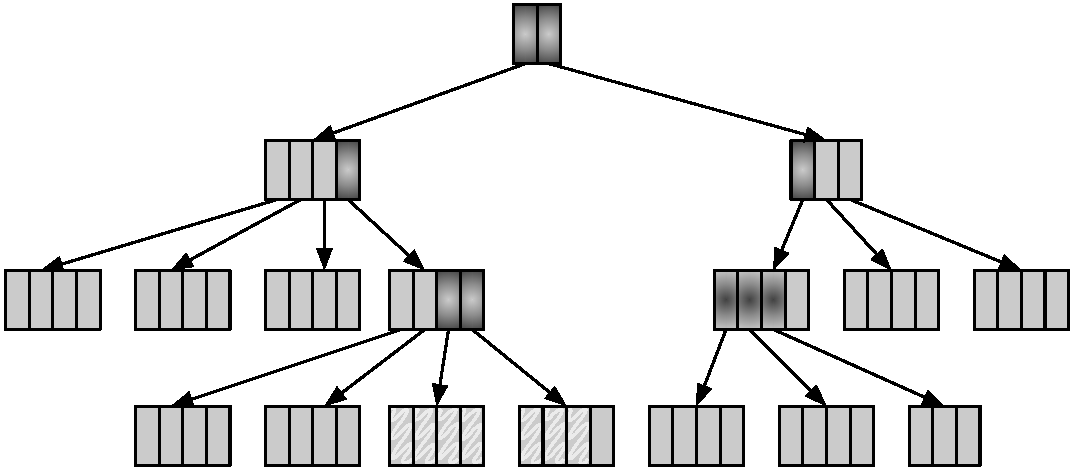
\includegraphics[width=0.8\textwidth]{Figures/Concat3.pdf}
  \caption{Concatenation example with blocks of size 4: Rebalancing level 3}
  \label{Concat3Benchmarks}
\end{figure}

% choose of algorithm
The concatenation algorithm chosen as for the RRB-Vector is the one that is slower but that rebalances better the trees. The reason behind this decision is that with better balanced trees all other operations on the trees are more performant. In fact choosing the least performant option does not need to be seen as a reduction in performance because the improvement is in relation to the RB concatenation linear complexity. An interesting consequence of the this choice, is that all vectors of size at most 1024\footnote{The maximum size of a two level RRB-Tree.} that where created by concatenation will be completely balanced.

% optimizations on small appends and prepends
When using displays and transient states, concatenating a small vector the concatenation algorithm is less performant that strait forward append or prepends on the other vector. That case is identified by using bounds on their lengths. If one is big and the other is small, a \texttt{prependAll}/\texttt{appendAll} variant is used. Those two operations are optimised version of the \texttt{append}/\texttt{prepend} that do not create the intermediate \texttt{Vector} wrapper object and some of the leaf arrays. When both vector are small enough the rebalance is done directly with \texttt{mergedLeafs}.

\paragraph{InsertAt}
% new operation
% describe simple implementation using split and concat 
% performance log_32 (from split + concat)
The operation \texttt{insertAt} is not currently defined on \texttt{Vector} because there is no way to implement it efficiently. But with RRB-Trees it is possible to implement this operation quite simply using \texttt{splitAt}, \texttt{append} and \texttt{concatenate}. This implementation has a time complexity of $log_{32}(n)$ that comes directly from the operations used.

\begin{lstlisting}[frame=single]
def insertAt(elem: A, n: Int): Vector[A] = {
  val splitted = this.splitAt(n)
  (splitted._1 :+ elem) ++ splitted._2
}
\end{lstlisting}

% hint at possible optimization by inserting directly and using transient states (take advantage of locality)
As this operation is new in the context of a vector and no real world use cases exist, this simple implementation is used. It would be is possible to optimise for localised inserts using displays and transient states.

\subsection{Prepend and Drop}
% describe different implementation
From a high level, the \texttt{prepend} and \texttt{drop} operations on RB-Trees and RRB-Trees are quite similar. The difference is in the way the nodes are copied, updated and cut. In the RRB operations the \texttt{startIndex} becomes zero when a node is not full the unbalanced nodes are used.

Both these operation will most of the time create new unbalanced nodes, but only on the left most branch. Calling several times combinations of these two will not contribute in generating even more unbalanced branches. As such they are only responsible for the creation of at most $ log_{32}(n)$ unbalanced nodes on any vector.

\paragraph{Prepend}
Just like with the RB version, the first step is to traverse down the left most part of the tree. Traversing the tree becomes trivial because now the first branch is alway on subindex 0. As know there is a need for checking if there is still space in the leftmost branch the prepend returns a result if it could prepend it on that subtree. 

When prepending an element on a subtree, if the element was added the parent nodes are updated with there corresponding sizes. If the element could not be prepend, then we check if the root of the current subtree has still space for another branch. If there is space a new branch is prepended on it, otherwise the prepend is delegated back to the parent node.

\begin{lstlisting}[frame=single]
def +:(elem: A): Vector[A] = {
  def prepended(node: Array[AnyRef], depth: Int) = {
    if (depth == 1) {
      Some(copyAndPrepend(node, elem))
    } else {
      prepended(node(0), depth-1) match {
        case Some(newChild) => 
          Some(copyAndUpdate(node, 0, newChild)))
        case None if canPrependBranchOn(node) => 
          Some(copyAndPrepend(node, newBranch(depth-1)))
        case _ => None
    }
  }
  def newBranch(depth: Int): Array[AnyRef] = {
    val newNode = new Array[AnyRef](2)
    newNode(0) = if (depth==1) elem else newBranch(depth-1)
    newNode
  }
  prepended(root, depth) match {
    case Some(newRoot) => new Vector(newRoot, depth, ...)  
    case None => 
      Vector(copyAndPrepend(root, newBranch(depth)), 
             depth+1, ...)
  }
}
\end{lstlisting}

Sizes updated in adding one to each size and in the case of \texttt{copyAndPrepend} additionally prepend a 1. Nodes on new branches do not need sizes as they are balanced, but they still need the empty slot.

% Talk about balancing
This operation will generate unbalanced nodes, but will not unbalance the tree each time the \texttt{prepend} operation is called. In fact it will only generate a new unbalanced node when prepending a new branch on a balanced subtree. Then will start filling that new branch up to the point where it becomes balanced. 

% performance
% hint the displays
Due to the update of all nodes in the first branch, the complexity of this operation is $O(log_{32}(n))$. This complexity can be amortized to constant time using displays with transient states for consecutive prepend operations on the vector (see section \ref{sec:DisplaysTransient}).

%----------------------------------

\paragraph{Drop}
% describe difference between the implementation (null and shift vs. cut and update size)

Like with the RB-Tree \texttt{drop} operation, the first step is to traverse down the tree to the cut index. The difference is that when cutting the nodes, instead of clearing the left side of the node the node is truncated and the the sizes adjusted. The sizes of the nodes get truncated at the same index and are adjusted. For each node the adjustment is equal to the number of nodes that will be dropped in the left of the subtree. This numbers is already part of the computation of the cut indices on each node. 

% performance
The computational complexity of any split operation is $O(log_{32}(n))$ due to the traversal and copy of nodes on the branch where the cut index is located.

%-----------------------------------
%	SUBSUBSECTION
%-----------------------------------

\subsubsection{Parallel Vector}
% Combine: trivial expansion from builder
%% heuristic: try to construct balanced trees 
% Split into subtrees two, take the nearest power of 32 to the half
The main difference between the RB and RRB parallel vectors is in the implementation of the combiner. This combiner is capable of combining in parallel and each combination is done in $O(log_{32}(n))$. The splitter also changed a bit to add an heuristic that helps on the performance of the combination and will tend to recreate balanced trees. 

\paragraph{Splitter}
The splitter heuristic consists in creating partitions of the tree that contain a number of elements equal to a multiple of a completely filled tree (i.e. $a \cdot 32^b$ elements). The splinter will always split into two new splitters that have a size that is as equivalent as possible taking into account the first rule. To do so, the mid point of the splitter elements is identified, the shifted to the next multiple of a power of 32. This way all nodes will be full and the subsequent concatenation rebalancing will be trivial. As all blocks are full, there is no node that requires shifting elements and therefore new block creation can be avoided.

\paragraph{Combiner}
The combiner is a trivial extension of the RRB-Vector builder. It wraps an instance of the builder and for each operation of the \texttt{Combiner} that is defined in \texttt{Builder} it delegates it to the builder. The \texttt{combine} operation concatenates the results of the two builders into a new combiner.

The advantages of this combiner are that the combination is done in $O(log_{32}(n))$ and they can't run in parallel on different thread of the thread pool.

